\part{Déroulement du stage}

\paragraph*{}
\lipsum[1]


\chapter{Projet OpenNebula}

\section{Premiers pas}

\paragraph*{}
Les premiers jours de mon stage ont été dédiés pour tester les logiciels OpenNebula et Xen sur une platforme de test
composée d'un petit serveur accueillant OpenNebula, de deux machines utilisées comme hyperviseurs Xen et d'un NetApp.
Vivien, pour responsable de stage, avait déjà déployé un environnement de développement fonctionnel sur ces machines.

\paragraph*{}
Afin de prendre en main la platforme, mon premier objectif à été de mettre à jour OpenNebula qui était en version 2.2 vers la version 3.0 Beta 1.
Cette version 2.2 a été modifié par Vivien pour fonctionner avec un plugin qu'il a écrit pour ajouter le support de l'iSCSI pour déporter le stockages des images
disque des VMs sur le NetApp.
\\
Il m'a donc fallu comprendre puis adapter le travail de Vivien. J'ai ensuite effectué beaucoup de tests pour valider le fonctionnement
de la nouvelle solution et aussi en valider ma compréhension.
\\
Après avoir compris comment marchait OpenNebula de l'extérieur - en tant qu'utilisateur - j'ai téléchargé les sources et ai préparé un
environnement de développement pour éditer, compiler\footnote{Étape de construction de l'exécutable du logiciel à partir des sources},
débugger\footnote{Action de compiler et lancer un exécutable d'une certaine manière permettant de voir le fonctionnement interne de l'application
pendant son fonctionnement pour comprendre et corriger des bugs}, installer et tester le logiciel.

\section{Interface de commande}
\paragraph*{}
OpenNebula peut être piloté via plusieurs interfaces:
\begin{listi}
	\item une interface web appelé Sunstone. voir figure \ref{sunstone}.
	\item une CLI\footnote{\index{CLI}CLI: \emph{Command Line Interface}, interface en ligne de commande}. voir \ref{clione}.
	\item une API\footnote{\index{API}API: \emph{Application Programming Interface}, Interface de programmation} de type
		XML\footnote{XML: \emph{Extensible Markup Language}, langage de balisage extensible, est un format de de structuration de donnée générique.}/RPC
		\footnote{RPC: \emph{Remote Procedure Call}, appel de procédure distant, est un protocole réseau fait pour appeler des procédure au sein d'un programme
		travers d'un réseau}
\end{listi}

\subsection{La CLI d'OpenNebula}
\label{onecli}

\subsubsection{L'affichage de la liste de tout les \emph{hosts}/hyperviseurs}
\begin{lstlisting}
oneadmin@opennebula:~$ onehost list
  ID NAME               RVM   TCPU   FCPU   ACPU   TMEM   FMEM   AMEM   STAT
   0 hyp1                 1    400    399    300     4G   2.7G   3.9G     on
   1 hyp2                 2    400    399    100     4G   1.2G   3.2G     on
\end{lstlisting}

\subsubsection{L'affichage de la liste des VMs}
\begin{lstlisting}
oneadmin@opennebula:~$ onevm list
ID USER     GROUP    NAME         STAT CPU     MEM        HOSTNAME        TIME
 0 oneadmin oneadmin vm1          runn   1    256M            hyp2 08 03:36:24
 1 oneadmin oneadmin vm2          runn   4   2048M            hyp2 00 00:01:38
 2 oneadmin oneadmin vm3          runn   2    128M            hyp1 00 00:01:00
\end{lstlisting}

\subsection{L'interface web Sunstone}

\begin{figure}[H]
\centering
\subfloat[\emph{Dashboard} / Tableau de bord]{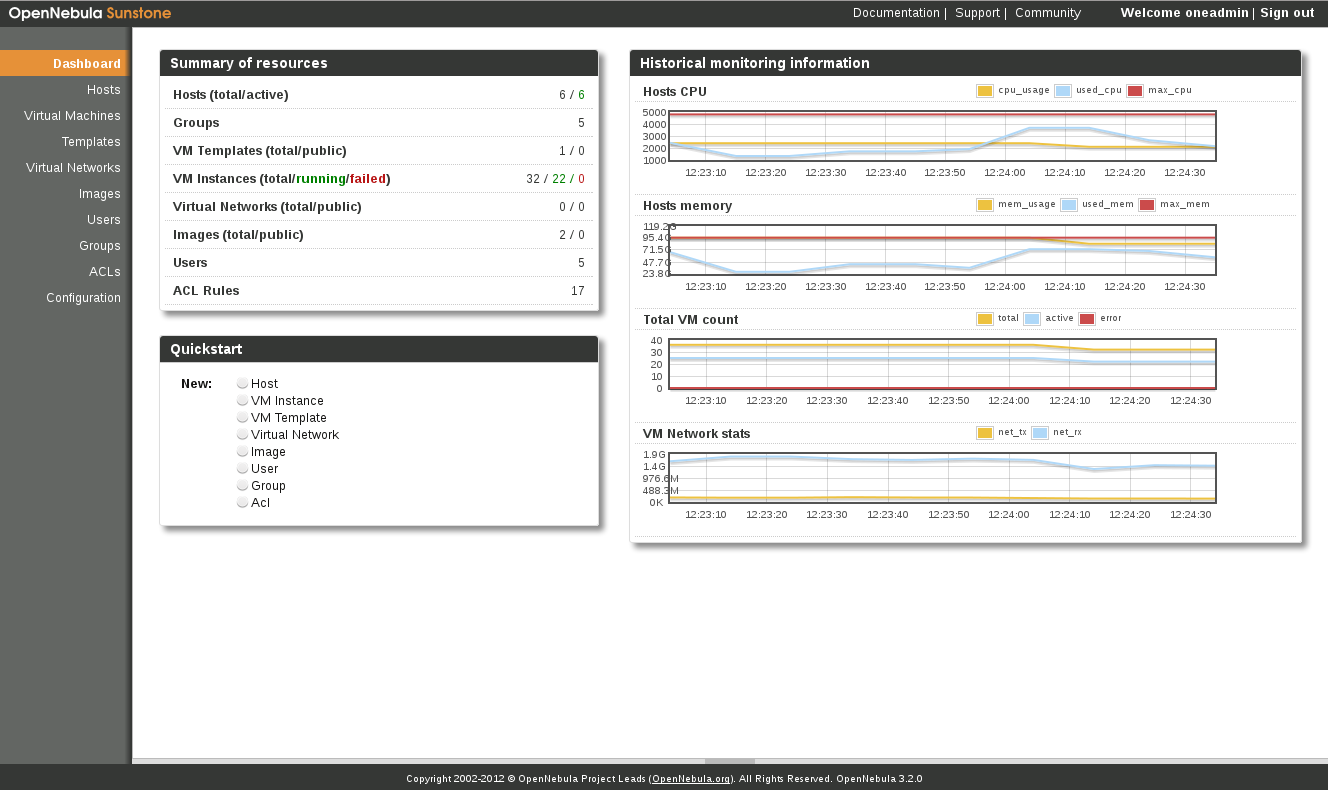
\includegraphics[width=0.5\textwidth]{resource/img/sunstone-dashboard}}
\subfloat[Création d'une VM]{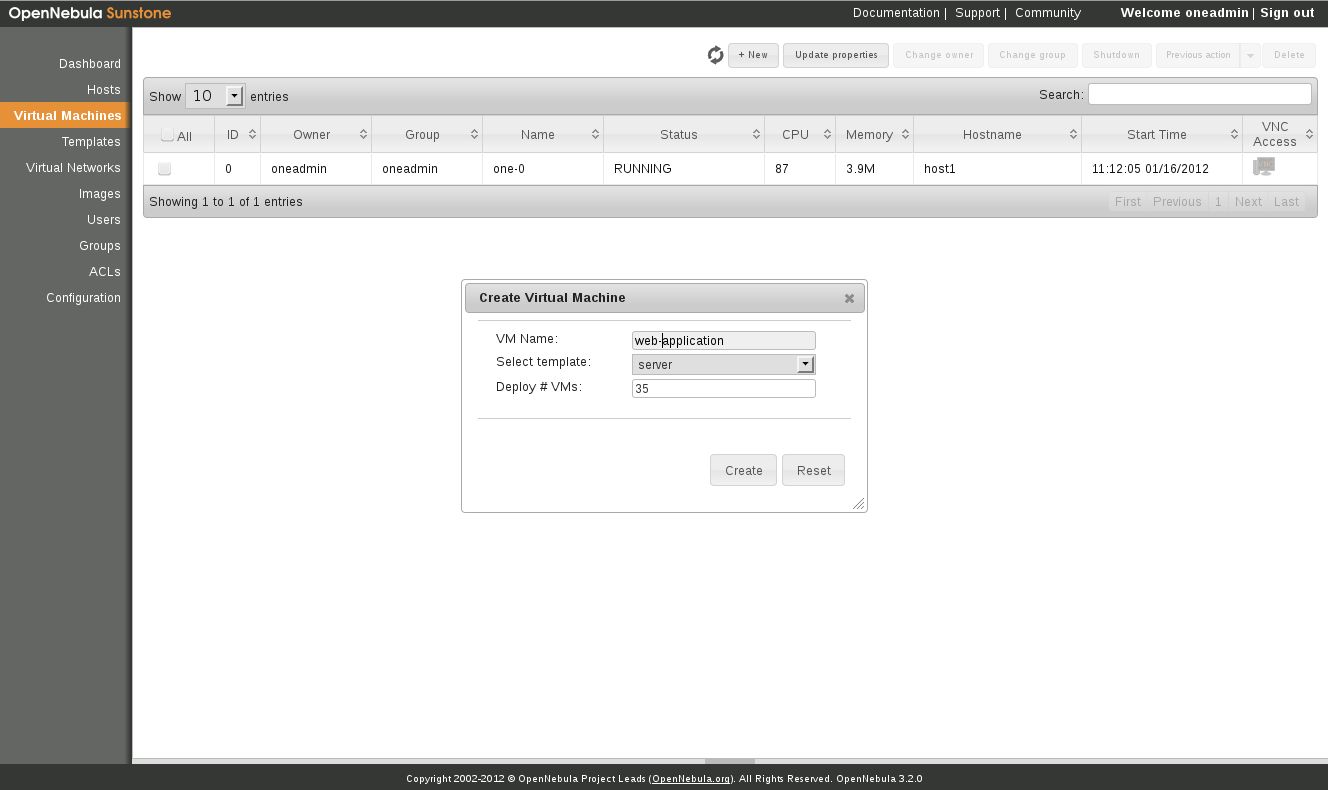
\includegraphics[width=0.5\textwidth]{resource/img/sunstone-createvm}}
\\
\subfloat[Création d'un template de VM]{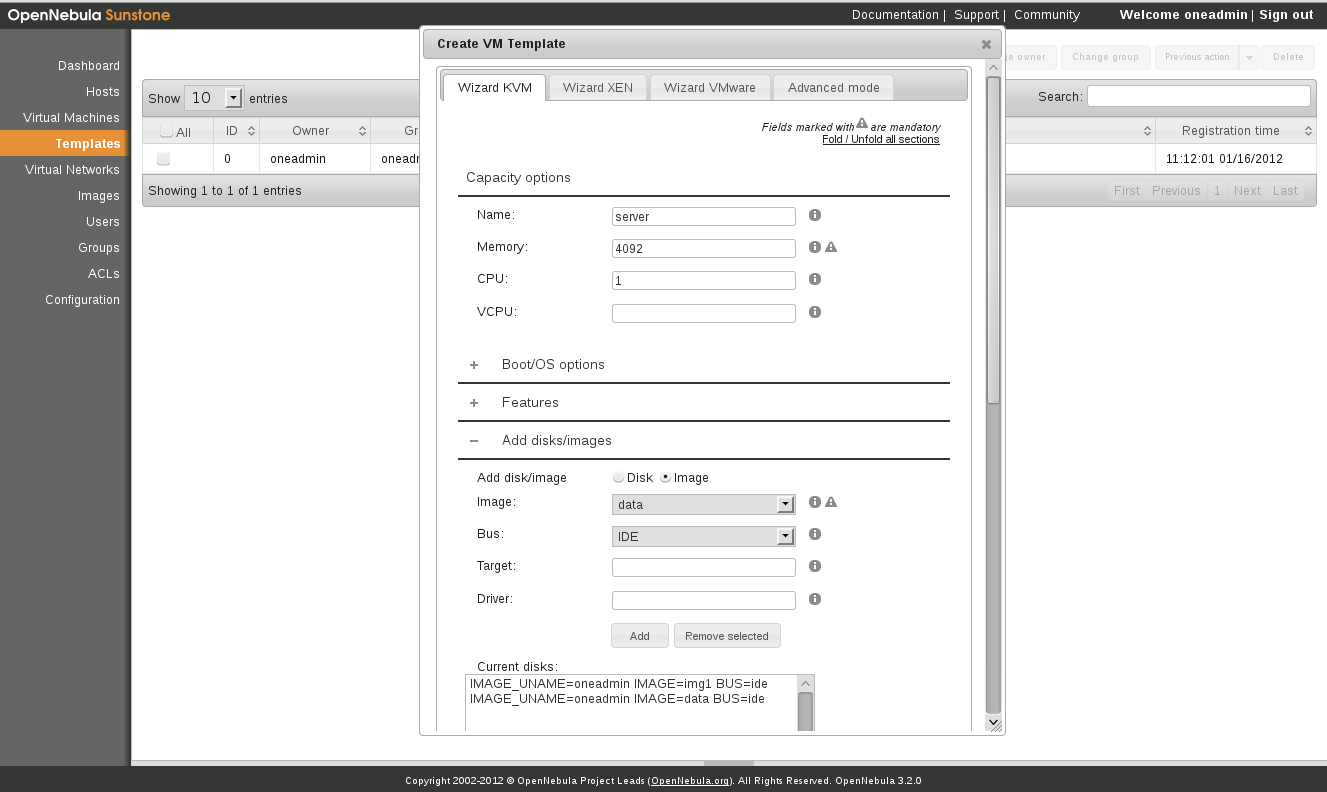
\includegraphics[width=0.5\textwidth]{resource/img/sunstone-createtemplate}}
\subfloat[Affichage de la liste des \emph{hosts}]{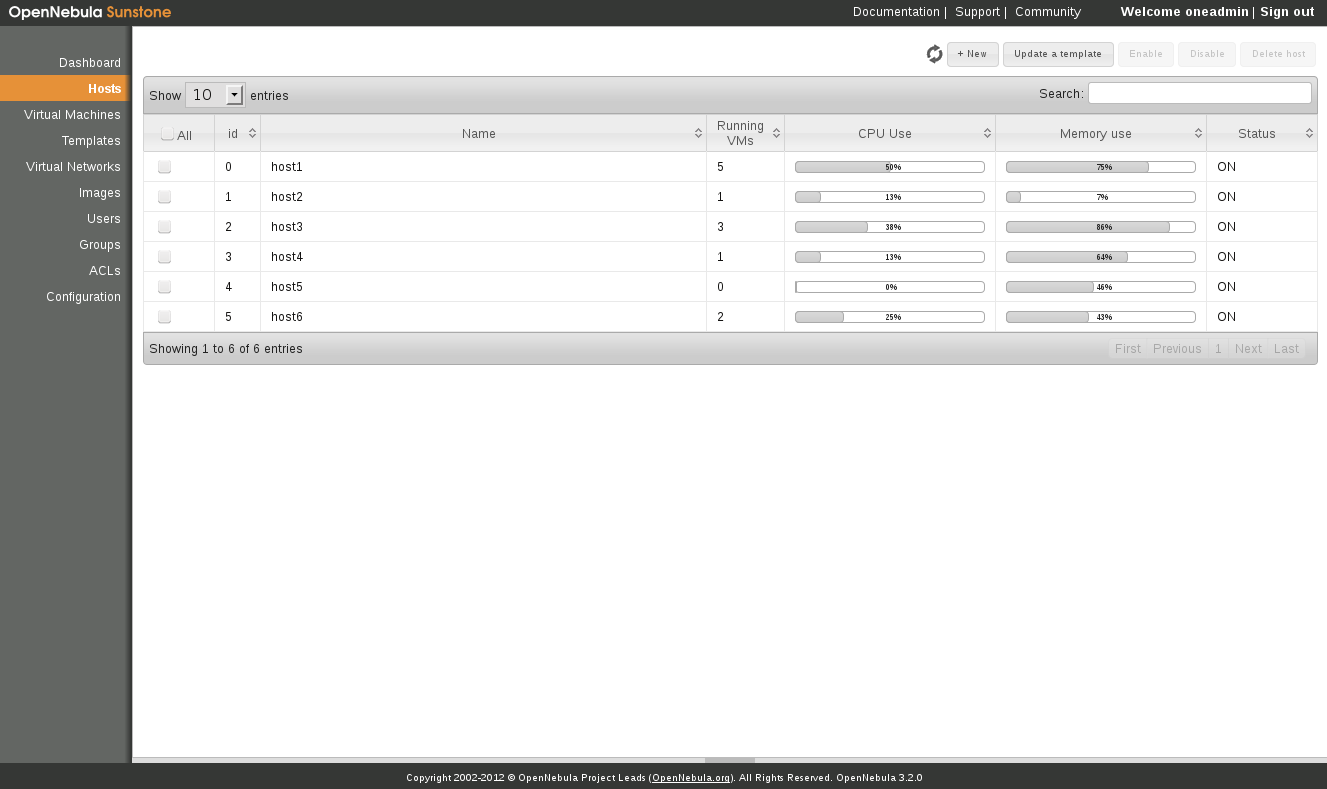
\includegraphics[width=0.5\textwidth]{resource/img/sunstone-hosts}}

\caption{L'interface web Sunstone d'OpenNebula}
\index{Sunstone}
\label{sunstone}
\end{figure}

\subsection{Architecture du code d'OpenNebula}
\paragraph*{}
Le code d'OpenNebula est designé comme une machine à état séparés en modules qui communiquent des ordres d'action de manière asynchrone.
\\
Chaques modules tourne dans le contexte d'un \emph{thread} et utilise une file d'attente FIFO\footnote{FIFO: \emph{First In First Out}, est une structure de donnée où les données poussées à l'interieur
en premier sont celles qui en sortent en premier aussi} pour recevoir les messages des autres \emph{threads} de manière asynchrone.

\paragraph*{}
La machine à état d'OpenNebula est principalement axé autour des états des VMs et plus précisément autour du lien entre les VMs et les \emph{Hosts}.


\section{L'environnement}

\paragraph*{}
Pour l'ajout des fonctions de \emph{scale-in}, j'ai du en même temps regarder ce qui était techniquement possible au niveau de l'hyperviseur Xen qui
sera utilisé comme backend\footnote{Un backend est la partie basse d'une architecture utilisé pour éffectuer des actions à l'extérieur du logiciel.
Par opposition le frontend est la partie haute de l'architecture recevant les ordres de l'utilisateur et commandant les autres parties de l'architecture}
par OpenNebula pour crééer les VMs sur un hyperviseur.

\paragraph*{}
En effet, en fonction des différentes version du noyau Linux et de Xen, certaines fonctionnalités sont disponibles, indisponibles ou buggés.\\
J'ai donc fait un tableau LibreOffice Calc\footnote{Logiciel open source concurrent de Microsoft\textsuperscript{\textregistered} Excel\texttrademark}
pour répertorier l'état de chaques fonctionnalités en fonction de toutes les combinaisons de versions possibles.
\\
Grâce à ce tableau, nous avons pu déterminer quelles étaient les fonctionnalités nous utiliserons et par déduction quelles versions de logiciels nous
installerons.

\paragraph*{}
Après avoir expérimenté avec la base de code d'OpenNebula nous avons fait des dessins d'architecture et une déterminé une procedure pour mettre en oeuvre ces
modifications.


\section{Nouvelle architecture}

L'objectif était de commencer par s'occuper des modifications de la gestion du stockage puis d'ajouter le support du \emph{scale in} qui est moins important.

\subsection{La gestion du stockage des images disque}
\paragraph*{}
Pour l'instant OpenNebula considère que les images disque des VMs sont soit stockées en local sur l'hyperviseur soit partagées sur un répertoire NFS
	\footnote{NFS: Network File System, est un système de fichier qui permet d'accèder à des fichiers via le réseau. Plusieurs clients peuvent accèder
	au mêmes fichiers en même temps. Ce système ressemble au protocole SMB de Microsoft\textsuperscript{\textregistered}}\index{NFS}
.
Vivien à aussi écrit un plugin OpenNebula pour partager les images disque via l'iSCSI - plus performant que le NFS pour ce type d'utilisation.
\\
Dans tout les cas, OpenNebula n'a pas été designé pour gérer plusieurs serveurs de stockage et répartir les images disque dessus.
\\
Les deux objets les plus important manipulés par OpenNebula sont les \emph{Hosts} et les VMs. Un \emph{Host} est le nom utilisé par OpenNebula pour
désigner un hyperviseur.
Un \emph{Host} contient donc zéro ou plusieurs VMs et une VM a forcément un et un seul \emph{Host} associé.


\paragraph*{}
Notre objectif serait de faire la même relation entre les images disques vs les serveurs de stockage et les VMs vs les \emph{Hosts}.
\\
OpenNebula n'a pour l'instant pas la notion de ce qu'est un serveur de stockage. Une image disque est juste un attribut d'une VM et n'a
pas de propriété faite pour désigner sur quel serveur de stockage elle se trouve.\\
De plus, par défault, OpenNebula considère que l'image disque d'une VM ne contient aucune donnée importante et est supprimée aussitôt
que la VM est détruite.

\paragraph*{}
Nous avons donc créé dans le code d'OpenNebula un nouveau type d'objet appelé \emph{storage backend}, littéralement << object s'occupant du stockage >>.
Un \emph{storage backend} pourra être un NetApp, un serveur NFS ou un cluster Ceph par exemple. Une image disque devient donc principalement un attribut d'un
\emph{storage backend} et peut vivre et être manipulées indépendement des VMs.\\


\paragraph*{}
Ce nouvelle object à nécéssité énormément de modifications au code source d'OpenNebula:
\begin{enumerate}
	\item Ajout de plusieurs modules pour gérer le cycle de vie d'un \emph{storage backend} et ses liens avec les autres objets du système.
	\item Designer un protocole de communication générique avec les driver/pilote des \emph{storage backend}.
	\item L'écriture d'une architecture de gestion de plugin/driver pour communiquer avec le \emph{storage backend} en question.
	\item Rédesigner entièrement et réécrire le \emph{Transfert Manager} (Gestionnaire de transfert) car il n'était pas du tout assez flexible
		pour gérer les tranferts entre différents \emph{storage backend}.
	\item Étendre le protocole XML/RPC et les outils de la CLI pour pouvoir administrer ces nouvelles fonctionnalités.
	\item Documenter les modifications
	\item Écrire des tests unitaires pour vérifier qu'il n'y a pas de régressions introduites.
\end{enumerate}

\section{Bilan}

\paragraph*{}








\chapter{Le projet H2O}



\chapter{Le projet Kanopya}

\section{Présentation}


\chapter{Autres travaux}

\section{Conférence OpenStack}

\section{Projet STERN}


\section{Déployement automatisé de site web Symfony 2}


\section{Déployement de Bacula sur FreeBSD et ZFS}


\begin{pygmented}{c}
void main(int argc, char* argv[])
{
	printf("hello");
	return 0;
}
\end{pygmented}

\cite{test}
